Implementation issues have been briefly discussed in \cite{cui_2016_scalcom}. 
In this paper we present the details of our full-feature implementation of lsMPI, which is a library for Message Passing Inteface. 
Instead of a building a complete MPI implementation from scratch, lsMPI is designed as a separate layer between MPI and user application, and uses the MPI profiling hooks to intercept every MPI call. In this way, we not only can take advantage of existing MPI performance optimization that numerous researches have spent years on, but also achieve portability across all MPI implementations that comply with the MPI standard.
When used, lsMPI transparanetly spawns the shadow processes during the initialization phase, manage the coordination between main and shadow processes during execution, and guarantee order and consistency for messages and non-deterministic events.
%Once completed, users should be able to link to the library without any change to existing codes. 

\subsection{Execution rate control}
While the mains always execute at maximum rate for the consideration of HPC's throughput goal, the shadows can be configured to executing slower by collocation \cite{cui_2016_scalcom}. When the user specifies $N$ processes, lsMPI will translate it into $2N + K$ processes where $K$ is the number of shadowed sets. The user has the flexibility to specify how the main processes are organized into shadowed sets through a rankfile. During initialization lsMPI will spawn $N$ main processes, $N$ shadow processes, and $K$ shadow coordinator processes for $K$ shadowed sets. The logical organization is depicted in Figure~\ref{fig:logical_org}. Each shadow coordinator is collocated with all the shadow processes in a shadowed set, and it manages the coordination between main and shadow processes the shadowed set. When a main process finishes, it will notify its corresponding shadow coordinator, which then terminates the associated shadow process to save power. When a main process fails, the shadow coordinator will send a signal to initiates a leaping from the associated shadow.  
%the RAS system will notify the corresponding shadow coordinator, which then promotes the associated shadow process to a new main process and kills the collocated shadows.

\begin{figure}[!t]
  \begin{center}
      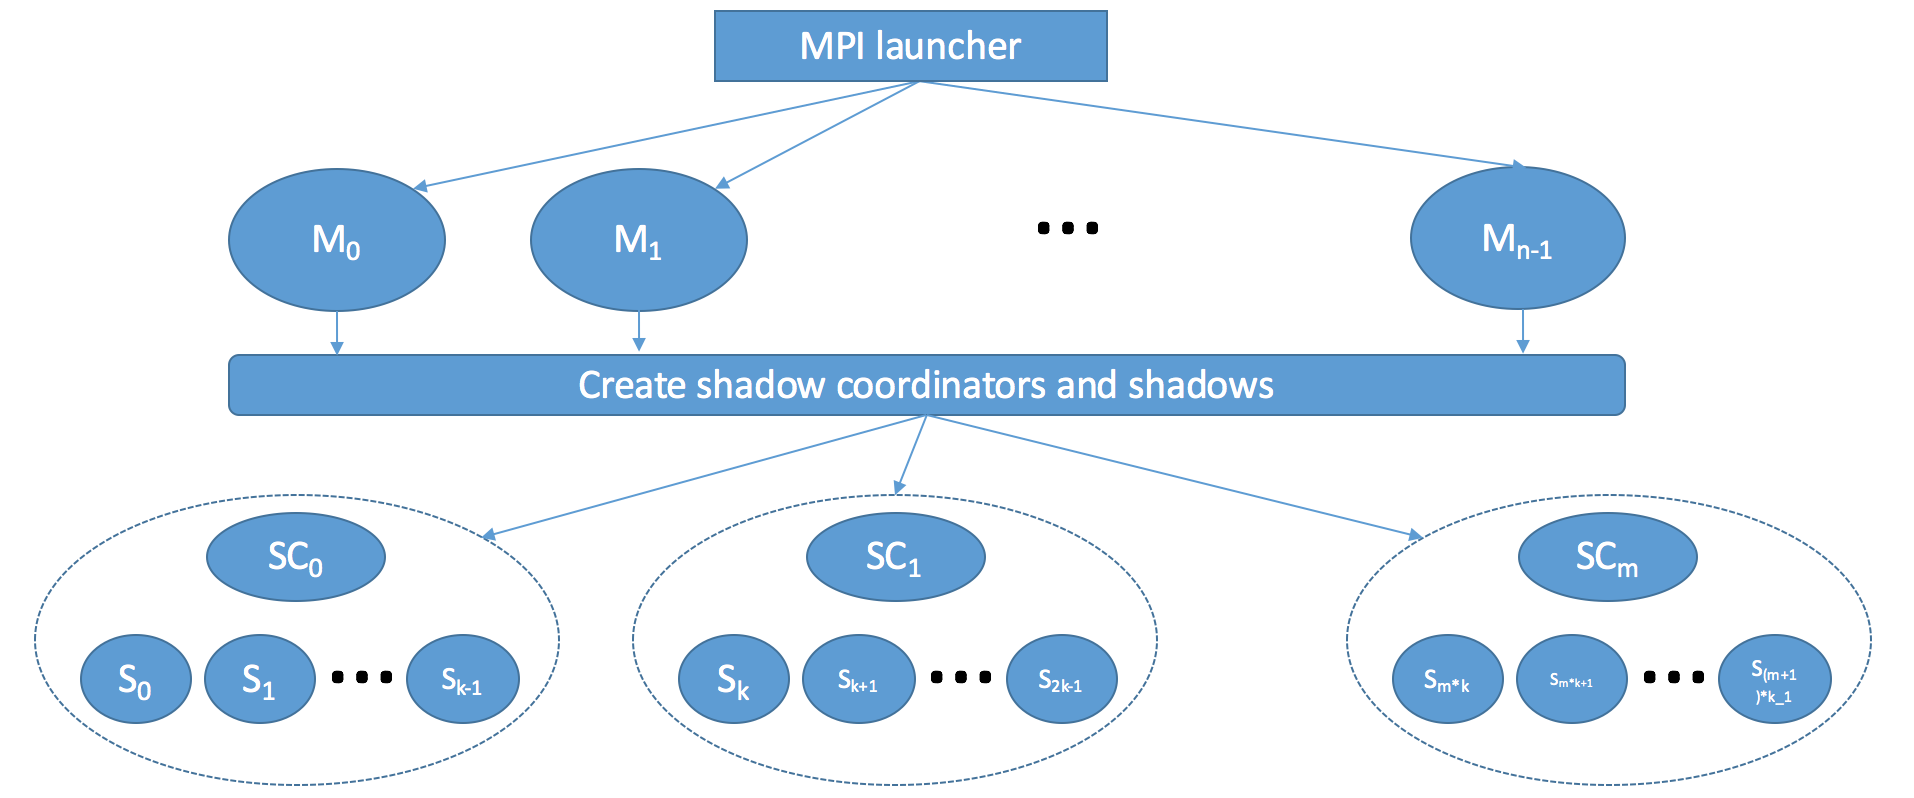
\includegraphics[width=\columnwidth]{figures/logical_org}
  \end{center}
  \caption{Logical organization of a MPI world with Lazy Shadowing.}
  \label{fig:logical_org}
\end{figure}

\subsection{Consistency}

State consistency between mains and shadows is required both during normal execution and following a failure. % of a main process to roll-forward the shadows. 
We design a consistency protocol, as shown in Figure~\ref{fig:cons_protocol}, 
to assure 
that the shadows see the same message order and MPI operation results as the mains. In this figure, A and B represent two mains, and A' and B' are their shadows. 
For each message, the main of the sender sends a copy of the message to each of the main and shadow of the receiver, and the shadow of the sender is suppressed from sending out messages. We assume that two copies of the same message are sent in an atomic manner, as this multicast functionality can be implemented within NIC. 


\begin{figure}[!t]
  \begin{center}
      	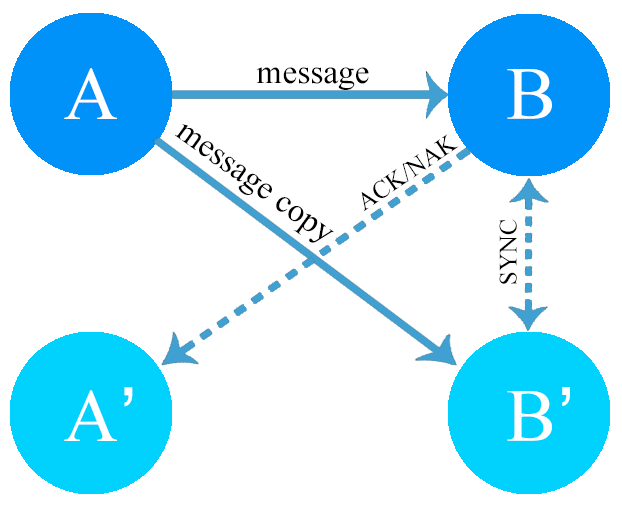
\includegraphics[width=0.7\columnwidth]{figures/cons_protocol}
  \end{center}
  %\vskip -0.25in
  \caption{Consistency protocol for lsMPI.}
  \label{fig:cons_protocol}
\end{figure}

We assume that only MPI operations can introduce non-determinism. MPI\_ANY\_SOURCE receives may result in different message orders between the main and shadow. To deal with this, we always let the main receive a message ahead of the shadow and then forward the message source to its shadow using a SYNC message (Figure~\ref{fig:cons_protocol}). 
The shadow then issues a receive with the specific source. Other operations, such as MPI\_Wtime() and MPI\_Probe(), can be dealt with by always forwarding the result from the main to the shadow.


\subsection{Leaping}
Checkpointing/restart requires each process to pause and save its execution state, which can be used by the same or a different process to update its state. Leaping is similar to Checkpointing/restart in saving a process' execution state, but the state is always transferred between a pair of main and shadow processes. 
To reduce the size of data involved in saving a process' execution state, we choose to implement leaping in the same way as application-level checkpointing. lsMPI provides a routine for users to register data as process state. Application user could use application specific knowledge to register only necessary variables, or use compiler techniques to automate this~\cite{5160999}. 

The function header for process state registration is as follows:

void leap\_register\_state(void *addr, int count, MPI\_Datatype dt);

For each piece of data to be registered, three parameters are needed: a pointer to the address of the data, the number of data items, and the datatype. Internally, lsMPI uses a linked list to keep track of all registered data. After each call of ``leap\_register\_state()", lsMPI will add a node to its internal linked list to record the three parameters. During leaping, the linked list is traversed to retrieve all registered data as the process state.

Coordination of leaping is easier than coordination of checkpointing, since leaping is always between a pair of main and shadow processes. To synchronize the leaping between a main and a shadow, shadow coordinator in the corresponding shadowed set is involved. For example, when a main process detects failure of another main process and decides to initiate a leaping, it will send a specil message to its shadow coordinator, which then uses a signal to notify the associated shadow to participate in the leaping. 

Different from Checkpointing where the process state is saved to storage, leaping directly transfers process state between a main and its shadow. 
Since lsMPI keeps track of the mapping between each main and its shadow and MPI provides natural support for message passing between processes, 
lsMPI uses MPI messages to transfer process state. Although multiple pieces of data can be registered as a process' state, only a single message is needed to transfer the process state, as MPI supports derived datatypes. To prevent the messages carrying process state from mixing with application messages, lsMPI uses a separate communicator for process state messages. With the synchronization of leaping by shadow coordinator and the fast transfer of process state via MPI messages, the overhead of leaping is minimized. 

A challenge in leaping lies in the need for maintainning state consistency across leaping. To make sure a pair of main and shadow stay consistent after a leaping, not only user-defined states should be transfered correctly, but also lower level states, such as program counter, need to be updated correspondingly. Specifically, the process which updates its process state during leaping needs to satisfy two requirements. Firstly, after updating its state, the process should resume execution at the same point as the process providing the state. Secondly, the process should discard obsolete message that previously stored in its buffer before resuming normal execution. To address this challenge, first we assume that the application's main body consists of a loop, which is true in most cases. 

To satisfy the first requirement, we restrict leaping to always occur at certain possible points, and uses internal counter to make sure that both main and shadow start leaping from the same point. For example, when a main process triggers a leaping and askes shadow coordinator to notify its associated shadow, the shadow coordinator will triggers the shadow's specific signal handler. The signal handler does not carry out leaping, but sets a flag for leaping and receives a counter value that indicates the leaping point from its main process. Then, the shadow will checks the flag and compare the counter value at every possible leaping point. Only when both the flag is set and counter value matches will the shadow start leaping. In this way, it is guaranteed that after leaping the main and shadow will resume execution from the same point. To balance the trade-off between the overhead and the flexibility of checking for when to perform leaping, we choose MPI receive operations as the possile points for leaping. 

There is no straighforward solution for the second problem as the message buffer is maintained by MPI runtime and not visible to lsMPI. Alternatively, we choose to remove obsolete message from message buffer by having the process execute all the skipped MPI communication routines after it finishes leaping. To achieve this, we require the user to define a function for the MPI communication functions used in the application's main body loop. The function should have two parameters to specify the starting and ending index for skipped iterations. In addition, the user needs to register the function with lsMPI with the following library call:

void leap\_register\_func(void (*func)(int, int));

To discard all obsolete messages after leaping, the process that updates its process state will call the registered function, for which the two parameters will be automatically specified by lsMPI. Essentially, it executes all the  MPI communication functions from the skipped iterations and consumes all the useless messages.  

%\subsection{Failure detection}
